\documentclass[letterpaper]{article} % DO NOT CHANGE THIS
\usepackage[preprint]{aaai2027} % DO NOT CHANGE THIS
% The serif, sans-serif, and monospaced fonts are loaded automatically by
% aaai2027.sty (newtxtext, helvet, courier). DO NOT add \usepackage{times},
% \usepackage{helvet}, \usepackage{courier}, or any other font package.
\usepackage[hyphens]{url}  % DO NOT CHANGE THIS
\usepackage{graphicx} % DO NOT CHANGE THIS
\urlstyle{rm} % DO NOT CHANGE THIS
\def\UrlFont{\rm}  % DO NOT CHANGE THIS
\usepackage{natbib}  % DO NOT CHANGE THIS AND DO NOT ADD ANY OPTIONS TO IT
\usepackage{caption} % DO NOT CHANGE THIS AND DO NOT ADD ANY OPTIONS TO IT
\frenchspacing  % DO NOT CHANGE THIS
%
% These are recommended to typeset algorithms but not required. See the subsubsection on algorithms. Remove them if you don't have algorithms in your paper.
\usepackage{algorithm}
\usepackage{algorithmic}
\usepackage{multirow}
%
% These are recommended to typeset listings but not required. See the subsubsection on listing. Remove this block if you don't have listings in your paper.
\usepackage{newfloat}
\usepackage{listings}
\DeclareCaptionStyle{ruled}{labelfont=normalfont,labelsep=colon,strut=off} % DO NOT CHANGE THIS
\lstset{%
	basicstyle={\footnotesize\ttfamily},% footnotesize acceptable for monospace
	numbers=left,numberstyle=\footnotesize,xleftmargin=2em,% show line numbers, remove this entire line if you don't want the numbers.
	aboveskip=0pt,belowskip=0pt,%
	showstringspaces=false,tabsize=2,breaklines=true}
\floatstyle{ruled}
\newfloat{listing}{tb}{lst}{}
\floatname{listing}{Listing}

%
% Recommended for better-looking tables
\usepackage{booktabs}
\usepackage{amsmath}
\usepackage{amssymb}
\newcommand{\model}{\textsc{SPEM}}
%
% Keep the \pdfinfo as shown here. There's no need
% for you to add the /Title and /Author tags.
\pdfinfo{
/TemplateVersion (2027.1)
}

% DISALLOWED PACKAGES
% \usepackage{authblk} -- This package is specifically forbidden
% \usepackage{balance} -- This package is specifically forbidden
% \usepackage{CJK} -- This package is specifically forbidden
% \usepackage{float} -- This package is specifically forbidden
% \usepackage{flushend} -- This package is specifically forbidden
% \usepackage{fullpage} -- This package is specifically forbidden
% \usepackage{geometry} -- This package is specifically forbidden
% \usepackage{hyperref} -- This package is specifically forbidden
% \usepackage{navigator} -- This package is specifically forbidden
% (or any other package that embeds links such as navigator or hyperref)
% \usepackage{indentfirst} -- This package is specifically forbidden
% \usepackage{layout} -- This package is specifically forbidden
% \usepackage{multicol} -- This package is specifically forbidden
% \usepackage{nameref} -- This package is specifically forbidden
% \usepackage{savetrees} -- This package is specifically forbidden
% \usepackage{setspace} -- This package is specifically forbidden
% \usepackage{stfloats} -- This package is specifically forbidden
% \usepackage{tabu} -- This package is specifically forbidden
% \usepackage{titlesec} -- This package is specifically forbidden
% \usepackage{tocbibind} -- This package is specifically forbidden
% \usepackage{ulem} -- This package is specifically forbidden
% \usepackage{wrapfig} -- This package is specifically forbidden
% DISALLOWED COMMANDS
% \nocopyright -- Your paper will not be published if you use this command
% \addtolength -- This command may not be used
% \balance -- This command may not be used
% \baselinestretch -- Your paper will not be published if you use this command
% \clearpage -- No page breaks of any kind may be used for the final version of your paper
% \columnsep -- This command may not be used
% \newpage -- No page breaks of any kind may be used for the final version of your paper
% \pagebreak -- No page breaks of any kind may be used for the final version of your paper
% \pagestyle -- This command may not be used
% \tiny -- This is not an acceptable font size.
% \vspace{- -- No negative value may be used in proximity of a caption, figure, table, section, subsection, subsubsection, or reference
% \vskip{- -- No negative value may be used to alter spacing above or below a caption, figure, table, section, subsection, subsubsection, or reference

\setcounter{secnumdepth}{0} %May be changed to 1 or 2 if section numbers are desired.

% The file aaai2027.sty is the style file for AAAI Press
% proceedings, working notes, and technical reports.
%

% Title

% Your title must be in mixed case, not sentence case.
% That means all verbs (including short verbs like be, is, using,and go),
% nouns, adverbs, adjectives should be capitalized, including both words in hyphenated terms, while
% articles, conjunctions, and prepositions are lower case unless they
% directly follow a colon or long dash
\title{SPEM: Structure-Aware Procedural Memory for Efficient Skill Use in LLM Agents}
\author{
    %Authors
    % All authors must be in the same font size and format.
    Written by AAAI Press Staff\textsuperscript{\rm 1}\thanks{With help from the AAAI Publications Committee.}\\
    AAAI Style Contributions by Peter Patel Schneider,
    Sunil Issar,\\
    J. Scott Penberthy,
    George Ferguson,
    Hans Guesgen,
    Francisco Cruz\equalcontrib\corresponding,
    Marc Pujol-Gonzalez\equalcontrib\corresponding
}
\author{
    Ran Zhou,
    Zehui Kong,
    Fanyu Lin,
    Jiaheng Liu,
    Zhen Zhang,
    Yuxiang Ren\corresponding
}
\affiliations{
    School of Intelligence Science and Technology, Nanjing University\\
    Correspondence: renyuxiang@nju.edu.cn
}



\begin{document}

\maketitle

\begin{abstract}
LLM-based agents increasingly rely on reusable skills. However, scaling skill libraries makes efficient and accurate skill use difficult. Full skill loading incurs high token and runtime overhead. In contrast, flat semantic retrieval treats skills as independent text entries, ignoring dependencies, execution order, state transitions, and data-flow constraints. We propose \model{}, a lightweight structure-aware procedural memory framework for efficient skill use in LLM-based agents. \model{} maintains Atomic Skill Memory for individual skills and Skill-DAG Memory for reusable compositions derived from successful executions. For a new task, \model{} reuses high-confidence Skill-DAG templates when available. Otherwise, it retrieves atomic skills and invokes Skill-GNN for state- and structure-aware skill selection. Successful executions are written back as new Skill-DAGs, allowing procedural memory to accumulate over time. Experiments on ALFWorld and SkillsBench show that \model{} achieves the best overall effectiveness--efficiency trade-off, reaching 87.1\% ALFWorld success and 38.38\% SkillsBench reward while reducing token and runtime costs against strong baselines.
\end{abstract}

% Uncomment the following to link to your code, datasets, an extended version or similar.
% You must keep this block between (not within) the abstract and the main body of the paper.
% Make sure that you do not de-anonymize yourself with these links.
% \begin{links}
%     \link{Code}{https://aaai.org/example/code}
%     \link{Datasets}{https://aaai.org/example/datasets}
%     \link{Extended version}{https://aaai.org/example/extended-version}
% \end{links}

\section{Introduction}

Large language model (LLM) agents are increasingly used as executable systems. They call tools, reuse skills, and interact with complex environments. In software engineering, data analysis, web automation, and embodied tasks, agents rely on reusable skills, such as file parsing, preprocessing, and API calling~\cite{schick2023toolformer,mialon2023augmented,yao2023react}. As skill libraries scale to hundreds or thousands of candidates, the central challenge changes. It shifts from whether useful skills exist to how an agent can retrieve, organize, and reuse the required skills efficiently~\cite{patil2023gorilla,qin2024toolllm,shi2025toolsavvy}.

Existing approaches face four limitations under large-scale skill libraries. First, loading all skill descriptions is infeasible due to high token cost,
context bloat, and runtime overhead, with important details often lost in long
contexts~\cite{liu2024lost}. Second, flat retrieval optimizes semantic relevance
but ignores structural dependencies like prerequisites, order, state
transitions, and data flow across skills~\cite{lewis2020rag,karpukhin2020dpr}.
Third, successful compositions are not stored as reusable procedural memory. Even
when dependency-aware plans are built, they are discarded after execution. This
forces agents to re-derive similar workflows~\cite{yao2023react,shinn2023reflexion}.
Finally, as agent systems are deployed more frequently and model capabilities continue to improve, efficiency becomes a primary concern. Repeated model invocations for retrieval, planning, and reorganization incur unnecessary token consumption, latency, and computational overhead. These limitations call for a framework that can retrieve skills compactly, organize them structurally, and accumulate reusable procedural memory over time.

We therefore study efficient skill use under large-scale skill
libraries. Our goal is to improve task success while reducing token cost,
runtime overhead, and repeated skill organization. To this end, we propose
\model{}, a lightweight structure-aware procedural memory framework. \model{}
maintains two complementary memory layers. Atomic Skill Memory represents
individual executable skills with their semantic, interface, and feedback
signals. Skill-DAG Memory stores reusable skill compositions distilled
from successful executions. Given a new task, \model{} first retrieves relevant
procedural memory and reuses a high-confidence Skill-DAG template when
available. Otherwise, or when the current guidance becomes insufficient,
Skill-GNN constructs a task-conditioned candidate graph. It then performs state-aware skill selection over retrieved atomic skills. After execution,
successful trajectories are compressed into Skill-DAGs and written back to
memory for future reuse.

We evaluate \model{} on SkillsBench and ALFWorld~\cite{li2026skillsbench,shridhar2020alfworld}.
SkillsBench tests large-scale skill retrieval and technical task execution. ALFWorld evaluates long-horizon dependencies, structured skill use, and
cross-task reuse in interactive environments. We compare \model{} with full
skill loading, flat vector retrieval, and graph-based skill selection baselines.

Our contributions are fourfold:
\begin{itemize}
    \item We propose \model{}, a dual-layer procedural memory framework that combines Atomic Skill Memory for fine-grained skill access with Skill-DAG Memory for reusable procedural structures.
    \item We design a Skill-GNN module for state-aware skill selection over task-conditioned candidate graphs.
    \item We introduce trajectory-DAG extraction to distill successful executions into reusable Skill-DAG templates and update procedural memory through execution feedback.
    \item We evaluate \model{} on ALFWorld and SkillsBench, achieving 87.1\% ALFWorld success and 38.38\% SkillsBench reward while reducing token and runtime costs over strong structure-aware baselines.
\end{itemize}

\section{Related Work}

\paragraph{From Tool Calling to Large-Scale Skill Retrieval.}
Early tool-augmented language models focused on tool invocation, argument generation, and reasoning with returned results. Pioneering works like ReAct, Toolformer, and surveys established the paradigm via reasoning-action interleaving, self‑supervised learning, and systematic analysis~\cite{yao2023react,schick2023toolformer,mialon2023augmented}. As external capabilities grow from a few tools to large API or skill libraries, retrieval becomes essential. Gorilla, API‑Bank, ToolBench, ToolLLM, and related methods reduce context overhead and calling errors through documentation retrieval, embedding, hierarchical search, task‑specific construction, or query rewriting~\cite{patil2023gorilla,li2023apibank,xu2023toolbench,qin2024toolllm,hao2023toolkengpt,du2024anytool,yuan2023craft,chen2024reinvoke}. However, most retrieval methods still treat capabilities as independent textual entries. They mainly optimize semantic relevance.
Skill retrieval is harder due to procedural knowledge, execution conditions, input‑output constraints, and task experience. Benchmarks like SkillsBench and SWE‑Skills‑Bench show that excessive or mismatched skills increase context cost and can hurt performance~\cite{li2026skillsbench,han2026sweskillsbench}. Thus, large‑scale skill use demands compact, relevant, and executable selection, not just semantic similarity.

\paragraph{From Structured Skills to Evolving Procedural Memory.}
As skills become reusable assets, recent work organizes them with explicit
structures. SkillNet represents skills through a unified ontology and relation
network. AgentSkillOS manages skills through classification, retrieval,
capability trees, and dynamic skill management~\cite{liang2026skillnet,li2026agentskillos}.
Graph-based methods further model relations among tools or skills. ToolNet
supports graph navigation over large tool collections; Graph of Skills retrieves
dependency-aware skill bundles from a skill dependency graph; and GraSP
constructs DAG-style skill structures with precondition and effect relations for
long-horizon tasks~\cite{liu2024toolnet,liu2026gos,xia2026grasp}. These methods
show that explicit structures help recover dependencies and execution relations. However, many of them use structure mainly for the
current task or as a static organization layer. They give limited attention to how
successful executions should be distilled, updated, and reused as evolving
procedural memory. \model{} instead converts successful trajectories into
reusable Skill-DAG templates and updates their reliability through execution
feedback.

\begin{figure*}[t]
  \centering
  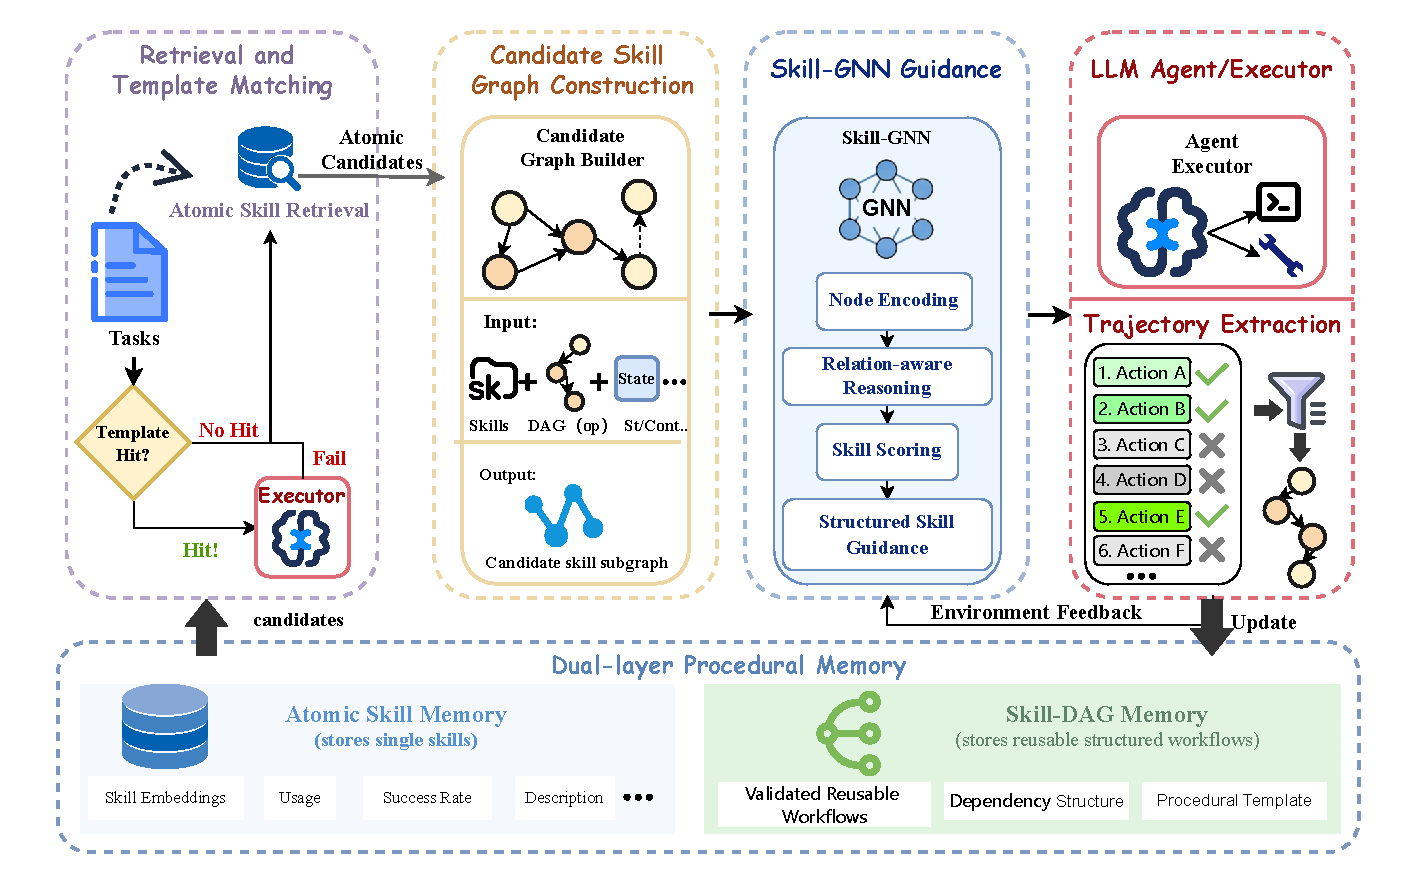
\includegraphics[width=0.9\textwidth]{Figures/skill-gnn.pdf} % Reduce the figure size so that it is slightly narrower than the column. Don't use precise values for figure width.This setup will avoid overfull boxes.
  \setlength{\abovecaptionskip}{0pt}
  \caption{Overview of \model{}. The system retrieves atomic skills or matched Skill-DAG templates from dual-layer procedural memory, constructs a task-conditioned candidate skill graph, and uses Skill-GNN to produce compact guidance for the LLM executor. Successful trajectories are distilled back into reusable Skill-DAG memory.}
  \label{framework}
\end{figure*}
  
\paragraph{Lightweight Skill Retrieval and Selection.}
Large-scale skill use imposes constraints on context, latency, and
computation. Recent work explores lightweight skill routing, representation, and
reuse. SkillRouter uses compact models for recall-then-rerank selection over
large skill sets. Formal Skill replaces verbose Markdown descriptions with
executable skill structures. CUA-Skill encapsulates GUI operation knowledge
into reusable skills for dynamic retrieval and parameter
instantiation~\cite{zheng2026skillrouter,zhang2026formalskill,chen2026cuaskill}.
Other methods emphasize reusable experience. ProcMEM converts interaction
experience into procedural memories. SkillDAG maintains typed relations among
skills and evolves across episodes. Compositional Skill Routing retrieves
skills for decomposed subtasks and composes them with a dependency-aware DAG
planner~\cite{mi2026procmem,bai2026skilldag,gao2026compositional}. These studies
show that lightweight skill use is not merely reducing retrieved skills, but
jointly concerns compact representation, efficient selection, execution
constraints, and experience reuse. \model{} addresses this gap through a unified
procedural memory framework that combines bounded atomic retrieval, reusable
Skill-DAG Memory, and Skill-GNN organization.

  
  \begin{figure*}[t]
      \centering
      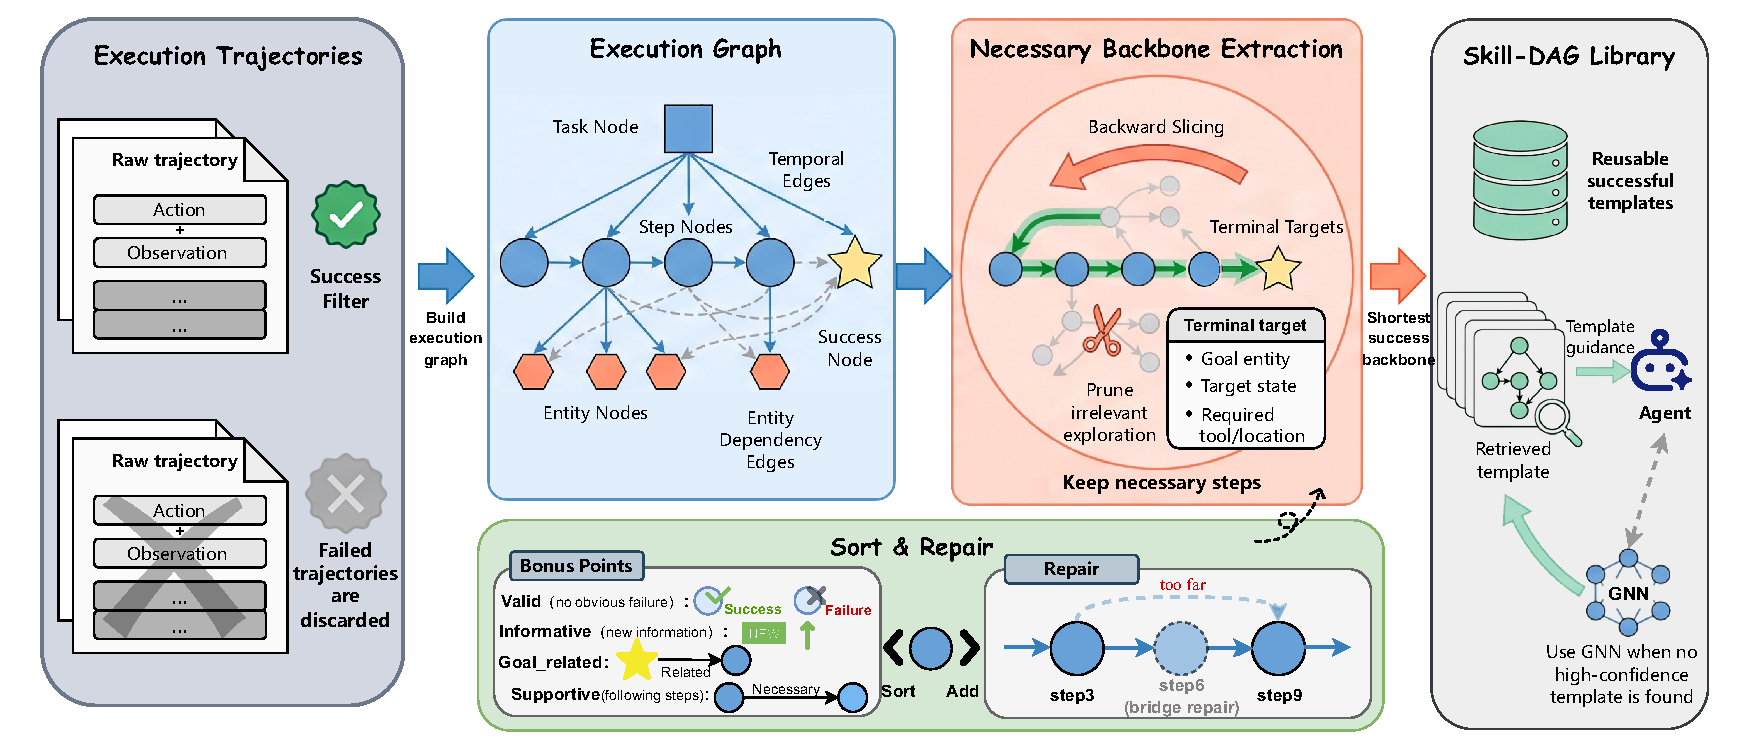
\includegraphics[width=\textwidth]{Figures/DAG.pdf}
      \setlength{\abovecaptionskip}{0pt}
      \caption{Overview of trajectory-DAG extraction. Successful trajectories are converted into execution graphs, from which necessary steps are identified through backward slicing, pruning, and dependency repair. The resulting backbones are stored as reusable Skill-DAG templates for future tasks.}
      \label{fig:trajectory_dag}
  \end{figure*}

\section{Method}

Given a task request and a large-scale skill library, \model{} provides compact,
executable skill guidance through two memory layers: Atomic Skill Memory for
individual skills and Skill-DAG Memory for reusable compositions distilled from
successful executions. As shown in Figure~\ref{framework}, \model{} reuses a
matched Skill-DAG template when available. Otherwise it retrieves atomic skills and invokes
Skill-GNN for state-aware reranking when needed. Successful executions are
written back as new Skill-DAGs. This enables procedural memory to accumulate over
time. The full protocol is provided in Section~A.1 of the supplementary material.

\subsection{Dual-Layer Procedural Memory}

\model{} separates procedural knowledge into two complementary memory layers. Atomic Skill Memory supports fine-grained access to individual skills, while Skill-DAG Memory supports direct reuse of successful skill compositions. The supplementary material provides the full schema and update rules in Section~A.2.

\paragraph{Atomic Skill Memory.}
Atomic Skill Memory represents each skill as a reusable executable unit rather
than an isolated text snippet. We denote it as
\begin{equation}
\mathcal{M}_{a}=\{s_i\}_{i=1}^{N},
\end{equation}
where each skill is represented as
\begin{equation}
s_i=(d_i,e_i,\sigma_i).
\end{equation}
Here, $d_i$ denotes skill metadata, $e_i$ denotes the semantic embedding.
$\sigma_i$ denotes lightweight execution feedback, such as usage frequency,
success rate, and execution cost. This allows retrieval to consider both semantic relevance and historical execution evidence without loading the full
skill library into the LLM context.

\paragraph{Skill-DAG Memory.}
Skill-DAG Memory stores reusable procedural templates extracted from successful
executions. We denote it as
\begin{equation}
\mathcal{M}_{d}=\{G_j\}_{j=1}^{M},
\end{equation}
where each Skill-DAG is represented as
\begin{equation}
G_j=(V_j,E_j,e_j,m_j).
\end{equation}
Here, $V_j$ contains procedural nodes, $E_j$ contains directed dependency edges,
$e_j$ is the task embedding associated with the template, and $m_j$ stores
compact execution metadata. A Skill-DAG captures a reusable execution structure. It allows the agent to reuse previously successful procedures instead of reconstructing them from scratch.

\paragraph{Procedural Memory Retrieval.}
Given a task request $q$, \model{} first searches Skill-DAG Memory for reusable templates:
\begin{equation}
\mathcal{C}_{d}(q)=
\{G_j \in \mathcal{M}_{d}\mid \operatorname{sim}(e_q,e_j)\geq \tau\},
\end{equation}
where $e_q$ is the task embedding and $\tau$ is the template matching threshold. If $\mathcal{C}_{d}(q)$ is non-empty, the highest-scoring Skill-DAG is injected as structured procedural guidance. If no template satisfies the threshold, \model{} retrieves a bounded set of atomic candidates:
\begin{equation}
\mathcal{C}_{a}(q)=
\operatorname{TopK}_{s_i\in\mathcal{M}_{a}}
\operatorname{sim}(e_q,e_i).
\end{equation}
The retrieved template or atomic candidates are then passed to the subsequent Skill-GNN orchestration stage when structure-aware organization is needed. This retrieval strategy avoids full-library loading while preserving two complementary modes of reuse: direct reuse of successful Skill-DAG templates and flexible organization of atomic skills for novel task states.


\subsection{Structure-Aware Skill Selection with Skill-GNN}

When reusable templates are unavailable or insufficient for the current execution context, \model{} uses Skill-GNN to perform structure-aware ranking and selection over retrieved atomic candidates. The goal is to identify semantically relevant skills. It also aims to select skills that are compatible with the task state and dependency relations among candidates.

\paragraph{Candidate Skill Graph Construction.}
Given a task request $q$, retrieved atomic candidates $\mathcal{C}_{a}(q)$, and
the current execution context, \model{} constructs a task-conditioned candidate
graph
\begin{equation}
\mathcal{G}_{q}=(\mathcal{V}_{q},\mathcal{E}_{q},\mathcal{R}),
\end{equation}
where $\mathcal{V}_{q}$ contains task, context, and candidate skill nodes.
$\mathcal{E}_{q}$ contains typed edges, and $\mathcal{R}$ denotes relation
types. Skill-node features combine semantic embeddings with lightweight
execution feedback. Task and context nodes encode the request, current
state, and execution history. Edges connect task--skill, context--skill, and
skill--skill pairs, capturing relevance, state compatibility, semantic
relatedness, and available dependency cues. Additional construction details are
provided in Section~A.5 of the
supplementary material.

\paragraph{Skill-GNN Scoring.}
Given $\mathcal{G}_{q}$, Skill-GNN first performs node encoding and relation-aware reasoning through message passing, as summarized in Figure~\ref{framework}. Let $h_i^{(0)}$ be the initial representation of node $i$. At layer $\ell$, the node representation is updated by aggregating messages from relation-specific neighbors:
\begin{equation}
h_i^{(\ell+1)} =
\phi_{\ell}\left(
h_i^{(\ell)},
\sum_{r \in \mathcal{R}}
\sum_{j \in \mathcal{N}_{r}(i)}
\alpha_{ij}^{r} W_{r}^{(\ell)} h_j^{(\ell)}
\right),
\end{equation}
where $\mathcal{N}_{r}(i)$ denotes neighbors of node $i$ under relation type $r$, $W_{r}^{(\ell)}$ is a relation-specific transformation. $\alpha_{ij}^{r}$ is the message weight, and $\phi_{\ell}$ is the layer update function.

After $L$ message-passing layers, Skill-GNN performs skill scoring. It assigns each candidate skill $s_i \in \mathcal{C}_{a}(q)$ a context-dependent utility score:
\begin{equation}
p_i=f_{\theta}\left(h_i^{(L)}\right).
\end{equation}
The top-ranked skills, together with compact dependency cues when available, are injected as structured guidance for the LLM agent. This graph-based scoring incorporates task relevance, runtime state, and inter-skill dependencies into the skill selection process.

\paragraph{Cold-Start Deployment.}
\model{} supports both trajectory-rich and trajectory-scarce deployment settings.
When target-domain trajectories are available, Skill-GNN is trained with
trajectory-prefix supervision, where each prefix defines the current procedural
state and the next executed skill is used as the target. When trajectories are
scarce or unavailable, \model{} uses a library-level warm start constructed only
from the skill library:
\begin{align}
\widetilde{\mathcal{D}}_{0}
&=
\{(\tilde{q}_{i}, s_i)\}_{s_i\in\mathcal{M}_{a}},\\
\widetilde{\mathcal{E}}_{0}
&=
\{(s_i,r,s_j)\mid \kappa_r(s_i,s_j)\ge \eta_r\},
\end{align}
where $\tilde{q}_{i}$ is a pseudo query generated from the metadata of skill
$s_i$, and $\widetilde{\mathcal{E}}_{0}$ contains weak skill--skill relations
induced by semantic similarity, shared tools, tags, or schema compatibility.
This initialization uses no task outcomes, verifier rewards, or evaluation
trajectories. During early deployment, Atomic Skill Memory retrieval and
available Skill-DAG templates provide the primary guidance, while the
warm-started Skill-GNN is used only for bounded reranking. As successful
executions accumulate, trajectory-DAG extraction converts them into new
Skill-DAG templates and trajectory-prefix training samples, gradually adapting
the system from retrieval-only guidance to state-aware graph selection. Since
Skill-GNN is inductive over dynamically constructed candidate graphs, it can
generalize to unseen tasks, unseen skill combinations, and newly extracted
Skill-DAG variants. Additional protocol and leakage-prevention details are
provided in Section~A.4 of the supplementary material.


\subsection{Trajectory-DAG Extraction}
As shown in Figure~\ref{fig:trajectory_dag}, \model{} converts successful interaction trajectories into reusable Skill-DAG templates after execution. Instead of storing complete trajectories, which may contain failed attempts, redundant exploration, or environment-specific details, the system extracts a compact execution backbone.  This backbone preserves the necessary steps for reaching the success condition. Given an execution trajectory $\tau$, the system first constructs an execution graph
\begin{equation}
G_{\tau}=(V_{\tau},E_{\tau}),
\end{equation}
where nodes represent executed steps and task-relevant states. Edges encode temporal order, entity dependencies, state transitions, and terminal reachability.

Starting from the successful terminal node $v_{\mathrm{succ}}$, the system performs backward slicing to identify success-relevant nodes:
\begin{equation}
V^{*}_{\tau}=\{v \in V_{\tau} \mid v \to^{*} v_{\mathrm{succ}}\},
\end{equation}
where $v \to^{*} v_{\mathrm{succ}}$ indicates that $v$ reaches the successful terminal state through temporal or dependency paths. Failed branches, redundant exploration, and operations that do not contribute to the final outcome are removed. The remaining nodes and their induced dependency edges are ordered and repaired according to temporal and dependency constraints, forming a compact Skill-DAG:
\begin{equation}
G^{*}_{\tau}=(V^{*}_{\tau},E^{*}_{\tau}).
\end{equation}
Finally, $G^{*}_{\tau}$ is written back to Skill-DAG Memory for future reuse. Successful non-template executions introduce new templates; successful template-guided executions reinforce or refine existing templates. Failed template executions only update reliability statistics. Detailed extraction rules, scoring signals, and update policies are provided in Section~A.3 of the supplementary material.

\section{Experiments}
\begin{table*}[t]
\centering
\small
\renewcommand{\arraystretch}{1.12}
\setlength{\tabcolsep}{5pt}
\begin{tabular}{llccc|cccc}
\toprule
\multirow{2}{*}{\textbf{Backbone}} &
\multirow{2}{*}{\textbf{Method}}
& \multicolumn{3}{c|}{\textbf{SkillsBench}}
& \multicolumn{4}{c}{\textbf{ALFWorld}}\\
\cmidrule(lr){3-5} \cmidrule(lr){6-9}
& & R $\uparrow$ & T $\downarrow$ & S $\downarrow$
& Success $\uparrow$ & Steps $\downarrow$ & Tokens $\downarrow$ & Runtime $\downarrow$ \\
\midrule

\multirow{5}{*}{\textbf{MiniMax-M2.7}}
& Vanilla Skills
& 21.61 & 798,323 & 469.3
& 59.3 & 21.24 & 152,242.1 & 55.95s \\
& Vector Skills
& 13.07 & \underline{722,765} & 439.5
& 63.9 & 18.36 & \underline{55,816.6} & 55.71s \\
& GoS
& 23.50 & 735,113 & \underline{399.4}
& \underline{68.6} & 20.26 & 62,033.9 & \underline{54.22s} \\
& SkillDAG
& \textbf{27.09} & 979,781 & 476.1
& 63.3 & \textbf{16.37} & 296,512.4 & 137.38s \\
& \textbf{Ours}
& \underline{25.14} & \textbf{721,926} & \textbf{360.5}
& \textbf{70.7} & \underline{18.29} & \textbf{45,785.7} & \textbf{51.56s} \\


\midrule

\multirow{5}{*}{\textbf{GPT-5.2-Codex}}
& Vanilla Skills
& 28.87 & 2,785,485 & \underline{686.8}
& 84.9 & \underline{14.65} & 99,023.9 & 84.57s \\
& Vector Skills
& 23.44 & \underline{1,047,698} & 763.4
& 83.7 & 16.18 & \textbf{47,357.3} & 80.43s \\
& GoS
& \underline{37.50} & 1,162,375 & 705.2
& 85.3 & 16.46 & 48,805.6 & \underline{71.23s} \\
& SkillDAG
& 34.38 & 1,370,270 & 861.1
& \underline{85.7} &\textbf{ 11.73} & 105,449.9 & 169.10s \\
& \textbf{Ours}
& \textbf{38.38} & \textbf{980,029} & \textbf{618.7}
& \textbf{87.1} & 15.07 & \underline{47,409.1} & \textbf{66.01s} \\


\bottomrule
\end{tabular}
\caption{Main results on SkillsBench and ALFWorld under different backbone models.
For SkillsBench, R denotes the verifier reward, T denotes average input tokens,
and S denotes agent-only runtime in seconds. For ALFWorld, Success denotes task
success rate, while Steps, Tokens, and Runtime denote average environment steps,
average token consumption, and agent-only runtime, respectively.
$\uparrow$ indicates higher is better, and $\downarrow$ indicates lower is better.
Bold numbers indicate the best result within each backbone group and benchmark,
and underlined numbers indicate the second-best result.}
\label{tab:main_results}
\end{table*}
\subsection{Experimental Setup}

\paragraph{Benchmarks.}
We evaluate \model{} on two complementary skill-use benchmarks.
\textbf{ALFWorld} \cite{shridhar2020alfworld} is an interactive text-based embodied environment. It requires multi-step household task completion, testing long-horizon dependencies, state transitions, and procedural reuse.
\textbf{SkillsBench} \cite{li2026skillsbench} evaluates technical agent tasks with large skill libraries. It tests whether agents can retrieve and apply task-relevant skills under limited context budgets.

\paragraph{Metrics.}
For ALFWorld, we report Success, Steps, Tokens, and Runtime.
Success ($\uparrow$) is the task success rate within the maximum step budget. Steps ($\downarrow$) is the average number of environment interactions. Tokens ($\downarrow$) is the average token consumption during agent execution, and Runtime ($\downarrow$) is the average agent-only execution time.

For SkillsBench, we report verifier reward $R$ ($\uparrow$), average input tokens $T$ ($\downarrow$), and agent-only runtime $S$ ($\downarrow$).
Following the benchmark protocol, $R$ is determined by the official verifier.
For fair accounting, $S$ measures the agent execution phase and excludes environment setup, dependency installation, Docker build time, and verifier runtime. For \model{}, online skill retrieval or reranking invoked during execution is included in the measured agent phase.

\paragraph{Baselines.}
We compare \model{} with four baselines that form a controlled progression in
skill access and structure awareness. 
\textbf{Vanilla Skills} loads the full
skill library, testing whether exhaustive context alone is sufficient.
\textbf{Vector Skills} retrieves top-$k$ skills by embedding similarity,
isolating the effect of flat semantic retrieval.
\textbf{GoS} serves as a
representative static graph-retrieval method, using a prebuilt skill graph to
retrieve structurally related skills. 
\textbf{SkillDAG} serves as a recent
sota baseline for dependency-aware skill selection with
a self-evolving graph structure.
\textbf{\model{} (Ours)} further introduces
dual-layer procedural memory, trajectory-DAG extraction, and on-demand
Skill-GNN reranking. These baselines allow us to distinguish gains from more
context, semantic retrieval, static graph structure, typed graph selection, and
reusable procedural memory.

\paragraph{Implementation Details.}
For fair comparison, all methods use the same benchmark splits, skill libraries, agent interface, execution environment, and verification protocol.
We evaluate with two backbone LLMs, MiniMax-M2.7 \cite{minimax2026m27} and GPT-5.2-Codex \cite{openai2025gpt52codex}, representing weaker and stronger model settings.

On \textbf{ALFWorld}, we use the dev split with 140 episodes and set the maximum number of environment steps to 30.
All skill-based methods use the same library of 37 \texttt{alfworld-*} skills.
\model{} builds Atomic Skill Memory from this library, constructs Skill-DAG Memory only from successful non-evaluation trajectories, and trains Skill-GNN with trajectory-prefix supervision under disjoint training and evaluation instances.

On \textbf{SkillsBench}, we follow the GoS execution setting with Docker-based environments, Harbor agent execution, verifier-based evaluation, at most two attempts per task, and two concurrent trials.
Following the benchmark convention, tasks that remain unresolved due to
infrastructure failures after the allowed retries are excluded rather than
counted as model failures, leaving the same 67 valid model tasks for all methods.
All methods use the same \texttt{skills\_200} skill library.
\model{} builds Atomic Skill Memory from the same library and applies library-level warm start plus Skill-GNN reranking.
Detailed hyperparameters, leakage-prevention rules, retry handling, and additional inference details are provided in Section~B of the supplementary material.

\begin{figure*}[t]
  \centering
  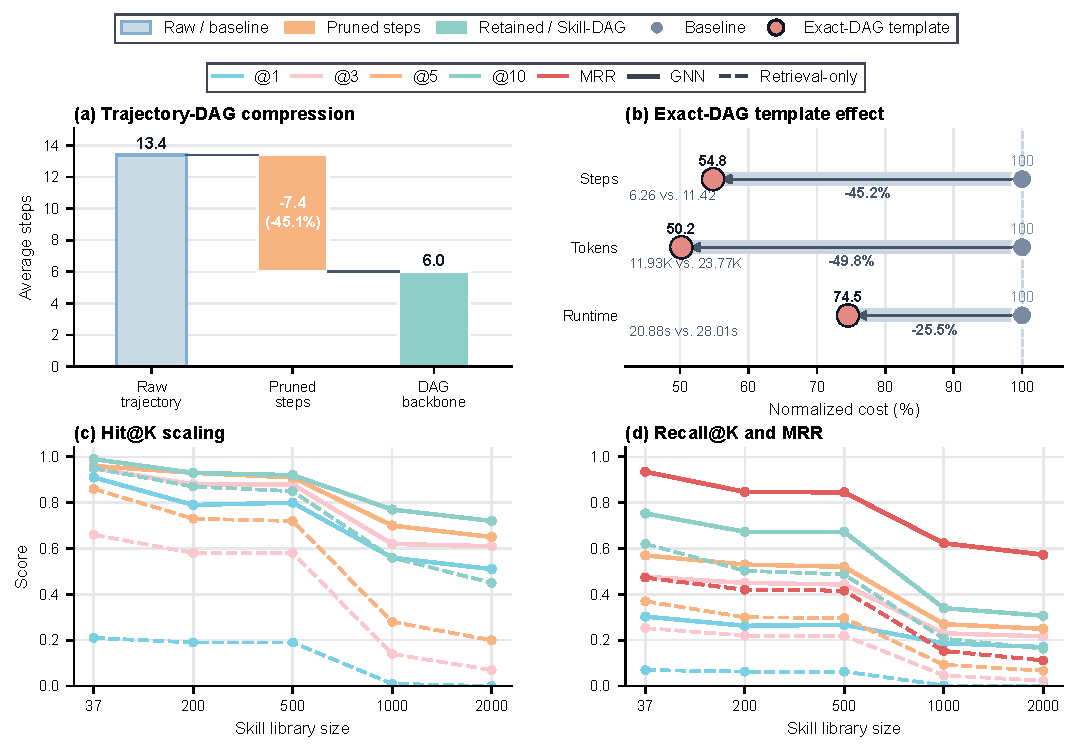
\includegraphics[width=0.75\textwidth]{Figures/effectiency.pdf}
  \setlength{\abovecaptionskip}{0pt}
  \caption{Effectiveness and scalability analysis.
(a) Trajectory-DAG extraction compresses successful trajectories into compact DAG backbones.
(b) Exact-DAG template reuse reduces normalized execution cost.
(c) Hit@K under different skill library sizes.
(d) Recall@K and MRR under different skill library sizes. Solid lines denote GNN-based reranking, while dashed lines denote retrieval-only selection.}
\label{fig:dag_scaling_analysis}
\end{figure*}
\subsection{Main Results}

\paragraph{Overall effectiveness--efficiency trade-off.}
Table~\ref{tab:main_results} shows that \model{} achieves the best overall
trade-off across both benchmarks and backbone models. On ALFWorld, \model{}
obtains the highest success rate under both MiniMax-M2.7 and GPT-5.2-Codex,
improving over GoS by 2.1 and 1.8 percentage points, respectively, while also
achieving the lowest runtime. On SkillsBench, \model{} achieves the best reward
with GPT-5.2-Codex and the second-best reward with MiniMax-M2.7, where SkillDAG
obtains a higher reward but requires substantially more tokens and runtime. In
particular, compared with SkillDAG under MiniMax-M2.7, \model{} reduces input
tokens by 26.3\% and runtime by 24.3\%, while remaining competitive in reward.

\paragraph{Efficiency becomes more important with stronger models.}
As the backbone model becomes stronger, structure-aware baselines such as GoS
and SkillDAG also obtain competitive rewards, especially on SkillsBench. This
makes efficiency a critical differentiator rather than a secondary metric.
Under GPT-5.2-Codex, \model{} improves SkillsBench reward over GoS from
37.50\% to 38.38\%, while reducing input tokens by 15.7\% and runtime by
12.3\%. On ALFWorld, SkillDAG achieves fewer steps, but it incurs much higher
token and runtime costs. In contrast, \model{} maintains the highest success
rate with much lower execution overhead, suggesting that reusable procedural
memory is most useful when it provides compact guidance rather than longer
plans or larger context.

\paragraph{Why structure matters.}
The comparison among Vector Skills, GoS, SkillDAG, and \model{} clarifies the
role of structure. Vector Skills often reduce context size but can lose
important procedural dependencies, leading to weaker reward or success. GoS and
SkillDAG show that explicit skill structures improve task performance, but they
mainly rely on static or pre-constructed structures and may introduce extra
context or execution overhead. \model{} further combines Atomic Skill Memory,
reusable Skill-DAG Memory, and state-aware Skill-GNN reranking, allowing the
agent to reuse successful procedural structures while keeping injected guidance
compact. These results indicate that the main advantage of \model{} is not
simply retrieving more skills, but selecting and reusing structured procedural
guidance under limited token and runtime budgets.

Detailed case analyzes of \model{} are provided in Section~D
of the supplementary material.

\begin{table}[t]
\centering
\small
\setlength{\tabcolsep}{4pt}
\renewcommand{\arraystretch}{1.08}
\begin{tabular}{lcccc}
\toprule
\textbf{Backbone} & \textbf{Hit} & \textbf{Fallback} & \textbf{Ineffective} & \textbf{Hit Success} \\
\midrule
\textbf{MiniMax-M2.7} & 56.43 & 43.57 & 25.32 & 74.68 \\
\textbf{GPT-5.2-Codex} & 60.71 & 39.29 & 14.12 & 85.88 \\
\bottomrule
\end{tabular}
\caption{Template-availability analysis on ALFWorld. All values are percentages.}
\label{tab:template_availability}
\end{table}
\subsection{Analysis of DAG-Template Effectiveness}
We analyze whether the extracted Skill-DAGs are both compact and useful.
As shown in Figure~\ref{fig:dag_scaling_analysis}(a), trajectory-DAG extraction
compresses successful trajectories from 13.4 average steps to 6.0 backbone
steps, pruning 54.9\% of operations while preserving the executable core.
This preliminarily demonstrates the compression effect of DAG templates.
We then evaluate the availability and effectiveness of DAG templates.
As shown in Table~\ref{tab:template_availability}, on ALFWorld, \model{}
achieves template hit rates of 56.43\% and 60.71\% under MiniMax-M2.7 and
GPT-5.2-Codex, respectively. Among template-hit tasks, the success rates are
74.68\% and 85.88\%, respectively. These results indicate that DAG templates can
accumulate reusable procedural structures for later tasks. Unlike ALFWorld,
SkillsBench contains highly heterogeneous technical tasks, where exact
procedural-template reuse is naturally limited. Therefore, we mainly use
SkillsBench to evaluate large-scale atomic-skill retrieval and structure-aware
reranking, and use ALFWorld to analyze Skill-DAG template reuse.
Finally, we conduct an exact-template analysis on ALFWorld. This isolates the effect of a correct DAG skeleton itself. For each successfully completed task, we
extract its trajectory and directly provide the DAG when re-executing
that task. This setting tests whether DAG templates can improve execution
efficiency. As shown in Figure~\ref{fig:dag_scaling_analysis}(b), exact-DAG
guidance preserves success on all evaluated tasks while reducing average steps
from 11.42 to 6.26, token consumption from 23.77K to 11.93K, and runtime from
28.01s to 20.88s, corresponding to reductions of 45.2\%, 49.8\%, and 25.5\%,
respectively. This suggests that templates provide effective procedural guidance
for improving task efficiency.


% Analyze Skill-DAG template hit rate, reuse benefit, token/runtime reduction,
% and performance under different library scales.

\begin{table}[htbp]
\centering
\small
\renewcommand{\arraystretch}{1.12}
\setlength{\tabcolsep}{3.8pt}
\begin{tabular}{lcccc}
\toprule
Method Variant & Succ. $\uparrow$ & Steps $\downarrow$ & Time $\downarrow$ & Tokens $\downarrow$ \\
\midrule
w/o Skill-DAG  & 56.8 & 23.0 & 55.4 & 67.5K \\
w/o Skill-GNN$^\dagger$ & 58.3 & 20.3 & 54.7 & 53.6K \\
w/o DAG Extraction & 63.0 & 18.9 & 57.8 & 56.2K \\
Full \model{} & \textbf{70.7} & \textbf{18.3} & \textbf{51.6} & \textbf{45.8K} \\
\bottomrule
\end{tabular}
\caption{Component ablation of \model{} on ALFWorld. Succ., Steps, Time, and Tokens denote task success rate, average completion steps, average runtime, and average token consumption. $^\dagger$ removes graph-based Skill-GNN and uses retrieved procedural memory.}
\label{tab:ablation}
\end{table}
\subsection{Ablation Study.}
\paragraph{\model{} Component Analysis}
Table~\ref{tab:ablation} evaluates the contribution of each component of \model{} on ALFWorld. 
\begin{itemize}
  \item \textbf{Skill-DAG templates} provide reusable procedural guidance. Removing them reduces success to 56.8\% and increases average steps to 23.0, indicating more redundant exploration. 
  \item \textbf{Skill-GNN} supports state-aware skill selection: without graph-based scoring, success drops to 58.3\%, showing that retrieved memory alone is not sufficient for stable execution under changing task states. 
  \item \textbf{DAG extraction} makes procedural memory compact. Replacing extracted Skill-DAG backbones with complete execution traces lowers success to 63.0\%. It also increases token and runtime cost, because full traces contain redundant exploration and environment-specific details. 
  \item \textbf{The full \model{}} achieves the best results across all metrics. This demonstrates that reusable Skill-DAG templates, structure-aware skill selection, and compact trajectory extraction are complementary.
\end{itemize}

\paragraph{Scalability to Larger Skill Libraries.}
Figures~\ref{fig:dag_scaling_analysis}(c) and (d) further examine whether structure-aware skill selection remains effective as the skill library grows. Retrieval-only selection degrades rapidly when the library size increases, especially at 1000 and 2000 skills, where semantic similarity alone struggles to rank the required skills near the top. In contrast, Skill-GNN consistently achieves higher Hit@K, Recall@K, and MRR across all library sizes. For example, at 2000 skills, Skill-GNN improves Hit@1 from 0.0 to 0.51 and MRR from 0.112 to 0.573 over retrieval-only selection. Although both methods become harder to rank as the candidate pool expands, the gap remains substantial, showing that graph-based contextualization helps preserve reliable skill selection under large-scale skill libraries.

Additional backbone comparisons and hyperparameter sensitivity analyses can be found in Section~C of the supplementary material.
% Remove Skill-DAG Memory, remove Skill-GNN, retrieval-only, no trajectory-DAG update,
% template-only / atomic-only variants.


\section{Conclusion}

We presented \model{}, a reusable and structure-aware skill memory framework for
LLM-based agents. Instead of treating skills as a flat prompt collection, \model{}
organizes them into Atomic Skill Memory for individual capabilities and
Skill-DAG Memory for reusable procedural structures. Skill-GNN further enables
state-conditioned skill selection over dynamically constructed candidate graphs, allowing the agent to adapt its guidance during execution while remaining inductive to new tasks and skill combinations.
Experiments on ALFWorld and SkillsBench show that \model{} improves both task effectiveness and execution efficiency across weaker and stronger backbone models. The results suggest that effective skill use requires more than semantic retrieval. Agents benefit from compact procedural guidance that captures both which skills are relevant and how they should be composed. Although current performance still depends on retrieval quality and the agent's ability to execute retrieved guidance, \model{} provides a practical step toward scalable, adaptive, and reusable skill memory for LLM-based agents.

\bibliography{aaai2027}

% Check whether the conference requires a reproducibility checklist to be included in the paper.
% If so, you can uncomment the following line and ajust the path to include it.
% \input{ReproducibilityChecklist.tex}

\end{document}
